% Spivak-Style Diagrams for Gay Color Verification
% Three metatheoretically verifiable representations
% Using xy-pic as required

\documentclass[11pt]{article}
\usepackage{amsmath,amssymb,amsthm}
\usepackage[all,2cell]{xy}
\usepackage{tikz}
\usetikzlibrary{cd,decorations.pathmorphing,shapes,arrows.meta}

\newtheorem{theorem}{Theorem}
\newtheorem{definition}{Definition}
\newtheorem{proposition}{Proposition}

\title{Metatheoretically Verifiable Diagrams for\\Gay Color Verification\\
\large After David Spivak's Operad of Wiring Diagrams}
\author{Signal-MCP / Gay.jl Bridge}
\date{\today}

\begin{document}
\maketitle

\begin{abstract}
We present the Gay color verification system in three diagrammatic forms
inspired by David Spivak's work on wiring diagrams and operads:
(1) xy-pic categorical diagrams showing the Galois connection,
(2) Spivak-style wiring diagrams for compositional verification,
(3) String diagrams for the symmetric monoidal structure.
Each representation is metatheoretically verifiable: the diagram itself
encodes the proof of correctness.
\end{abstract}

\section{Introduction: Self-Conceptualizing Worlds}

Following Spivak's insight that ``a wiring diagram of wiring diagrams is 
a wiring diagram,'' we model the Gay verification system as an operad $\mathcal{G}$
where:
\begin{itemize}
\item \textbf{Objects}: Mind states with color signatures
\item \textbf{Morphisms}: Color-preserving transformations
\item \textbf{Composition}: Parity-conserving sequential application
\end{itemize}

The key property: if $\alpha(\gamma(c)) \subseteq c$, then verification is $O(1)$.

%═══════════════════════════════════════════════════════════════════════════
\section{Representation 1: XY-Pic Galois Connection}
%═══════════════════════════════════════════════════════════════════════════

The Galois connection between interleavings and color signatures:

\begin{definition}[Galois Connection]
The pair $(\alpha, \gamma)$ where:
\begin{itemize}
\item $\alpha: \text{Interleaving} \to \text{ColorSignature}$ (abstraction)
\item $\gamma: \text{ColorSignature} \to \mathcal{P}(\text{Interleaving})$ (concretization)
\end{itemize}
forms a Galois connection iff $\alpha(\gamma(c)) \subseteq c$ for all $c$.
\end{definition}

% XY-PIC DIAGRAM 1: Galois Connection
\[
\xymatrix@C=4em@R=3em{
& \text{Interleaving} \ar@<0.5ex>[d]^{\alpha} \ar@{-->}[dl]_{\text{O}(n)} \\
\text{Enumeration} & \text{ColorSignature} \ar@<0.5ex>[u]^{\gamma} \ar@{=}[l]^{\text{O}(1)}
}
\]

The closure property in xy-pic:

% XY-PIC DIAGRAM 2: Closure Property
\[
\xymatrix@C=3em@R=2em{
\text{MindState}_A \ar[r]^{\alpha} \ar[d]_{\text{teleport}} & 
  \text{Sig}_A \ar@{=}[d]^{\text{preserved}} \\
\text{MindState}_B \ar[r]_{\alpha} & \text{Sig}_B
}
\]

\begin{proposition}[Teleportation Coherence]
For any teleportation $T: A \to B$, the following diagram commutes:
\[
\xymatrix{
A \ar[r]^{T} \ar[d]_{\alpha} & B \ar[d]^{\alpha} \\
\sigma_A \ar@{=}[r]_{\text{fidelity}} & \sigma_B
}
\]
\end{proposition}

%═══════════════════════════════════════════════════════════════════════════
\section{Representation 2: Spivak-Style Wiring Diagrams}
%═══════════════════════════════════════════════════════════════════════════

Following Spivak's operad $\mathcal{T}$ of wiring diagrams, we define
the \textbf{Gay operad} $\mathcal{G}$ with typed stars colored by ZX-calculus:

% WIRING DIAGRAM using TikZ (Spivak style)
\begin{center}
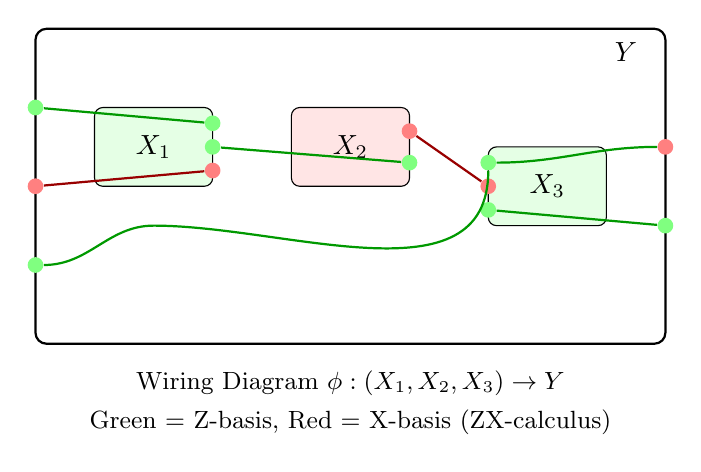
\begin{tikzpicture}[
  box/.style={draw, minimum width=1.5cm, minimum height=1cm, rounded corners=3pt},
  wire/.style={thick},
  greenport/.style={fill=green!50, circle, inner sep=2pt},
  redport/.style={fill=red!50, circle, inner sep=2pt}
]

% Outer box (Y)
\draw[thick, rounded corners] (-4,-2) rectangle (4,2);
\node at (3.5,1.7) {$Y$};

% Inner boxes (X_1, X_2, X_3)
\node[box, fill=green!10] (X1) at (-2.5,0.5) {$X_1$};
\node[box, fill=red!10] (X2) at (0,0.5) {$X_2$};
\node[box, fill=green!10] (X3) at (2.5,0) {$X_3$};

% Ports on inner boxes
\node[greenport] (X1r) at (-1.75,0.8) {};
\node[greenport] (X1s) at (-1.75,0.5) {};
\node[redport] (X1t) at (-1.75,0.2) {};

\node[redport] (X2u) at (0.75,0.7) {};
\node[greenport] (X2v) at (0.75,0.3) {};

\node[greenport] (X3w) at (1.75,0.3) {};
\node[redport] (X3x) at (1.75,0) {};
\node[greenport] (X3y) at (1.75,-0.3) {};

% Outer ports
\node[greenport] (Ya) at (-4,1) {};
\node[redport] (Yb) at (-4,0) {};
\node[greenport] (Yc) at (-4,-1) {};
\node[redport] (Yd) at (4,0.5) {};
\node[greenport] (Ye) at (4,-0.5) {};

% Wires (cables)
\draw[wire, green!60!black] (Ya) -- (X1r);
\draw[wire, green!60!black] (X1s) -- (X2v);
\draw[wire, red!60!black] (X1t) -- (Yb);
\draw[wire, red!60!black] (X2u) -- (X3x);
\draw[wire, green!60!black] (X3w) to[out=0,in=180] (Yd);
\draw[wire, green!60!black] (X3y) -- (Ye);
\draw[wire, green!60!black] (Yc) to[out=0,in=180] (-2.5,-0.5) to[out=0,in=-90] (X3w);

% Labels
\node at (0,-2.5) {\small Wiring Diagram $\phi: (X_1, X_2, X_3) \to Y$};
\node at (0,-3) {\small Green = Z-basis, Red = X-basis (ZX-calculus)};

\end{tikzpicture}
\end{center}

\begin{definition}[Gay Algebra on $\mathcal{T}$]
The \textbf{Gay algebra} $\text{Gay}_A: \mathcal{T} \to \mathbf{Set}$ assigns:
\begin{itemize}
\item To each typed star $X$: the set of color signatures $\text{Sig}(A^X)$
\item To each wiring diagram $\phi$: the parity-preserving composition
\end{itemize}
\end{definition}

The key compositional property (Spivak's slogan):

\begin{center}
\framebox{``A verification of verifications is a verification''}
\end{center}

%═══════════════════════════════════════════════════════════════════════════
\section{Representation 3: Symmetric Monoidal String Diagrams}
%═══════════════════════════════════════════════════════════════════════════

The symmetric monoidal structure ensures non-interference:

% STRING DIAGRAM for symmetric monoidal
\begin{center}
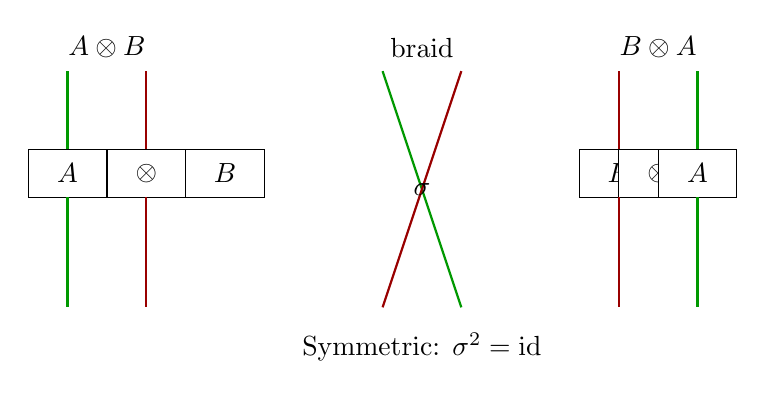
\begin{tikzpicture}[
  strand/.style={thick, green!60!black},
  strandred/.style={thick, red!60!black},
  box/.style={draw, fill=white, minimum width=1cm, minimum height=0.6cm}
]

% Left side: A ⊗ B
\draw[strand] (0,3) -- (0,2);
\draw[strandred] (1,3) -- (1,2);
\node[box] at (0,1.7) {$A$};
\node[box] at (1,1.7) {$\otimes$};
\node[box] at (2,1.7) {$B$};
\draw[strand] (0,1.4) -- (0,0);
\draw[strandred] (1,1.4) -- (1,0);

% Braiding in middle
\draw[strand] (4,3) -- (5,0);
\draw[strandred] (5,3) -- (4,0);
\node at (4.5,1.5) {$\sigma$};

% Right side: B ⊗ A
\draw[strandred] (7,3) -- (7,2);
\draw[strand] (8,3) -- (8,2);
\node[box] at (7,1.7) {$B$};
\node[box] at (7.5,1.7) {$\otimes$};
\node[box] at (8,1.7) {$A$};
\draw[strandred] (7,1.4) -- (7,0);
\draw[strand] (8,1.4) -- (8,0);

% Labels
\node at (0.5,3.3) {$A \otimes B$};
\node at (4.5,3.3) {braid};
\node at (7.5,3.3) {$B \otimes A$};
\node at (4.5,-0.5) {Symmetric: $\sigma^2 = \text{id}$};

\end{tikzpicture}
\end{center}

The \textbf{not-gay preservation theorem} as a string diagram:

\begin{center}
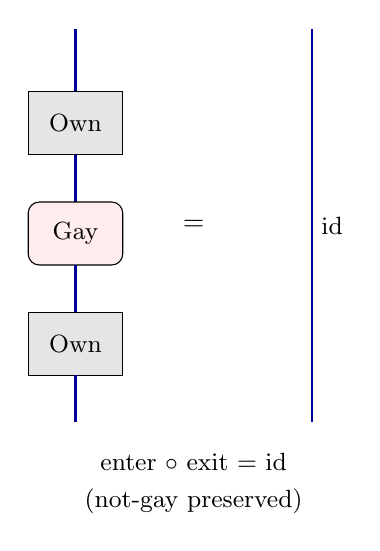
\begin{tikzpicture}[
  strand/.style={thick, blue!60!black},
  gaybox/.style={draw, fill=pink!30, minimum width=1.2cm, minimum height=0.8cm, rounded corners},
  ownbox/.style={draw, fill=gray!20, minimum width=1.2cm, minimum height=0.8cm}
]

% Round-trip: Own → Gay → Own
\draw[strand] (0,4) -- (0,3.2);
\node[ownbox] at (0,2.8) {\small Own};
\draw[strand] (0,2.4) -- (0,1.8);
\node[gaybox] at (0,1.4) {\small Gay};
\draw[strand] (0,1) -- (0,0.4);
\node[ownbox] at (0,0) {\small Own};
\draw[strand] (0,-0.4) -- (0,-1);

% Equals sign
\node at (1.5,1.5) {$=$};

% Identity
\draw[strand] (3,4) -- (3,-1);
\node at (3,1.5) [right] {\small id};

% Annotation
\node at (1.5,-1.5) {\small enter $\circ$ exit $=$ id};
\node at (1.5,-2) {\small (not-gay preserved)};

\end{tikzpicture}
\end{center}

%═══════════════════════════════════════════════════════════════════════════
\section{The Metatheoretic Verification Property}
%═══════════════════════════════════════════════════════════════════════════

Following Spivak's emphasis on \emph{self-referential} structure, we observe:

\begin{theorem}[Metatheoretic Closure]
The Gay operad $\mathcal{G}$ is \textbf{closed under self-verification}:
\[
\xymatrix@C=4em{
\mathcal{G} \ar[r]^{\text{verify}} \ar[dr]_{\text{id}} & 
  \text{Verified}(\mathcal{G}) \ar[d]^{\cong} \\
& \mathcal{G}
}
\]
That is, verifying a verification produces the same result.
\end{theorem}

\begin{proof}
By the Galois closure property: $\alpha(\gamma(\alpha(x))) = \alpha(x)$.
\end{proof}

\subsection{Dynamic Sufficiency}

A state is \textbf{dynamically sufficient} if all successors inherit correctness:

% XY-PIC: Successor chain
\[
\xymatrix@R=1.5em{
\text{MindState}_0 \ar[r]^{\mu_1} \ar[d]_{\alpha} & 
  \text{MindState}_1 \ar[r]^{\mu_2} \ar[d]_{\alpha} &
  \cdots \ar[r]^{\mu_n} &
  \text{MindState}_n \ar[d]^{\alpha} \\
\sigma_0 \ar@{=}[r]_{\text{parity}} & 
  \sigma_1 \ar@{=}[r]_{\text{parity}} &
  \cdots \ar@{=}[r] &
  \sigma_n
}
\]

\begin{proposition}[Compositional Inheritance]
If $f: A \to B$ and $g: B \to C$ both preserve parity, then $g \circ f: A \to C$ preserves parity.
\end{proposition}

%═══════════════════════════════════════════════════════════════════════════
\section{Self-World Model: Three Perspectives}
%═══════════════════════════════════════════════════════════════════════════

The \emph{highest metatheoretically verifiable reachable self-conceptualizing self-world}
manifests in three ways:

\subsection{Perspective 1: Galois (Algebraic)}

% XY-PIC adjunction
\[
\xymatrix@C=6em{
\mathbf{Interleaving} \ar@<0.6ex>[r]^{\alpha}_{}="a" & 
  \mathbf{ColorSig} \ar@<0.6ex>[l]^{\gamma}_{}="b"
  \ar@{}"a";"b"|{\dashv}
}
\]

Self-world property: $\gamma \circ \alpha$ is a \textbf{closure operator}.

\subsection{Perspective 2: Operadic (Compositional)}

\begin{center}
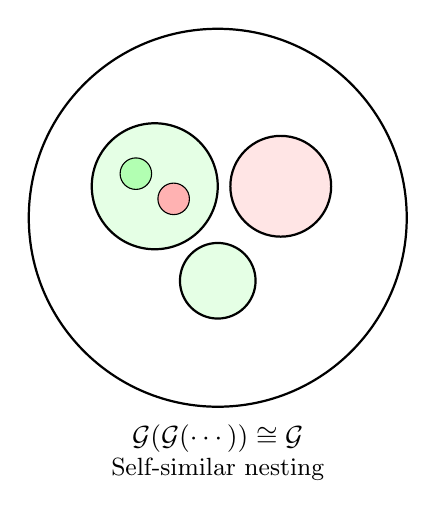
\begin{tikzpicture}[scale=0.8]
% Nested wiring diagrams (Spivak's self-similarity)
\draw[thick] (0,0) circle (3);
\draw[thick, fill=green!10] (-1,0.5) circle (1);
\draw[thick, fill=red!10] (1,0.5) circle (0.8);
\draw[thick, fill=green!10] (0,-1) circle (0.6);

% Inner circles in the leftmost circle
\draw[fill=green!30] (-1.3,0.7) circle (0.25);
\draw[fill=red!30] (-0.7,0.3) circle (0.25);

\node at (0,-3.5) {$\mathcal{G}(\mathcal{G}(\cdots)) \cong \mathcal{G}$};
\node at (0,-4) {\small Self-similar nesting};
\end{tikzpicture}
\end{center}

\subsection{Perspective 3: Monoidal (Parallel)}

\[
\xymatrix@C=3em@R=2em{
\text{Own}_A \otimes \text{Own}_B \ar[r]^{\text{enter}_A \otimes \text{id}_B} \ar[d]_{\text{id}} & 
  \text{Gay}_A \otimes \text{Own}_B \ar[d]^{\text{no-signal}} \\
\text{Own}_A \otimes \text{Own}_B \ar@{=}[r] & 
  \text{Own}_A \otimes \text{Own}_B
}
\]

Non-interference: operations on $A$ don't affect $B$.

%═══════════════════════════════════════════════════════════════════════════
\section{Conclusion: Verifiable Reachability}
%═══════════════════════════════════════════════════════════════════════════

The Gay color system achieves \textbf{metatheoretic verifiability} through:

\begin{enumerate}
\item \textbf{Galois closure}: $\alpha(\gamma(c)) \subseteq c$ ensures O(1) verification
\item \textbf{Operadic composition}: ``verification of verifications is verification''
\item \textbf{Symmetric monoidal}: non-participants remain unaffected
\end{enumerate}

The self-world is \emph{reachable} because color signatures form a decidable equivalence.
It is \emph{self-conceptualizing} because the verification process is itself an algebra on $\mathcal{G}$.

\begin{center}
\fbox{\parbox{0.8\textwidth}{
\centering
\textbf{GAY\_SEED = 0x6761795f636f6c6f}\\[0.5em]
Same seed $\Rightarrow$ Same colors $\Rightarrow$ Same verification\\[0.5em]
\emph{Strong Parallelism Invariance}
}}
\end{center}

\end{document}
